%! suppress = MultipleIncludes
%! Author = tom.koptel
%! Date = 31/10/2020

% Preamble
\documentclass[11pt]{article}

%Ukrainian-specific packages
%--------------------------------------
\usepackage[T2A]{fontenc}
\usepackage[utf8]{inputenc}
\usepackage[ukrainian]{babel}
%--------------------------------------

%Graphics-specific packages
\usepackage{graphicx}
\graphicspath{ {../images//} }

%Code-specific snippets
%--------------------------------------
\usepackage{listings}
\usepackage{xcolor}

\definecolor{codegreen}{rgb}{0,0.6,0}
\definecolor{codegray}{rgb}{0.5,0.5,0.5}
\definecolor{codepurple}{rgb}{0.58,0,0.82}

\lstdefinestyle{light}{
commentstyle=\color{codegreen},
keywordstyle=\color{magenta},
numberstyle=\tiny\color{codegray},
stringstyle=\color{codepurple},
basicstyle=\ttfamily\footnotesize,
breakatwhitespace=false,
breaklines=true,
captionpos=b,
keepspaces=true,
numbers=left,
numbersep=5pt,
showspaces=false,
showstringspaces=false,
showtabs=false,
tabsize=2
}

\lstset{style=light}
%--------------------------------------

%Hyphenation rules
%--------------------------------------
\usepackage{hyphenat}
\hyphenation{ма-те-ма-ти-ка вос-ста-нав-ли-вать}
%--------------------------------------

\title{Titanic Case study}
\author{Коптель Aртем Олегович}
\date{Листопад 2020}

% Document
\begin{document}

    \section{Data}\label{sec:data}
    \begin{center}
        \begin{tabular}{ |p{3cm}|p{4cm}|p{4cm}| }
            \hline
            survival & Survival                                    & 0 = No, 1 = Yes                                \\
            \hline
            pclass   & Ticket class                                & 1 = 1st, 2 = 2nd, 3 = 3rd                      \\
            \hline
            embarked & Port of Embarkation                         & C = Cherbourg, Q = Queenstown, S = Southampton \\
            \hline
            sex      & Sex                                         &                                                \\
            \hline
            Age      & Age in years                                &                                                \\
            \hline
            sibsp    & \# of siblings / spouses aboard the Titanic &                                                \\
            \hline
            parch    & \# of parents / children aboard the Titanic &                                                \\
            \hline
            ticket   & Ticket number                               &                                                \\
            \hline
            fare     & Passenger fare                              &                                                \\
            \hline
            cabin    & Cabin number                                &                                                \\
            \hline
        \end{tabular}
    \end{center}


    \section{Assumptions}\label{sec:assumptions}

    \subsection{All female passengers survived.}\label{subsec:first_assumption}

    \begin{lstlisting}[style=light, language=Python,label={lst:vectorimg},caption=Testing first assumption]
        women = train_data.loc[train_data.Sex == 'female']["Survived"]
        rate_women = sum(women)/len(women)
        print("% of women who survived:", rate_women)
        # % of women who survived: 0.7420382165605095

        men = train_data.loc[train_data.Sex == 'male']["Survived"]
        rate_men = sum(men)/len(men)

        print("% of men who survived:", rate_men)
        # % of men who survived: 0.18890814558058924
    \end{lstlisting}

    From this you can see that almost 75\% of the women on board survived, whereas only 19\% of the men lived to tell about it.


    \section{Intro to Machine Learning.}\label{sec:intro_to_ml}

    \subsection{Decision Tree.}\label{subsec:decision_tree}
    We use data to decide how to \underline{break} the houses into two (see image 1) \underline{groups}, and then again to determine the predicted price in each group.
    This step of capturing patterns from data is called \textbf{fitting} or \textbf{training} the model.
    The data used to \textbf{fit} the model is called the \textbf{training data}.

    You can capture more factors using a tree that has more "splits." These are called \textbf{"deeper" trees}.
    A decision tree that also considers the total size of each house's lot might look like on the image 2.

    The predicted price for the house is at the bottom of the tree.
    The point at the bottom where we make a prediction is called a \textbf{leaf}.

    \begin{figure}
        \label{fig:image2}
        \centering
        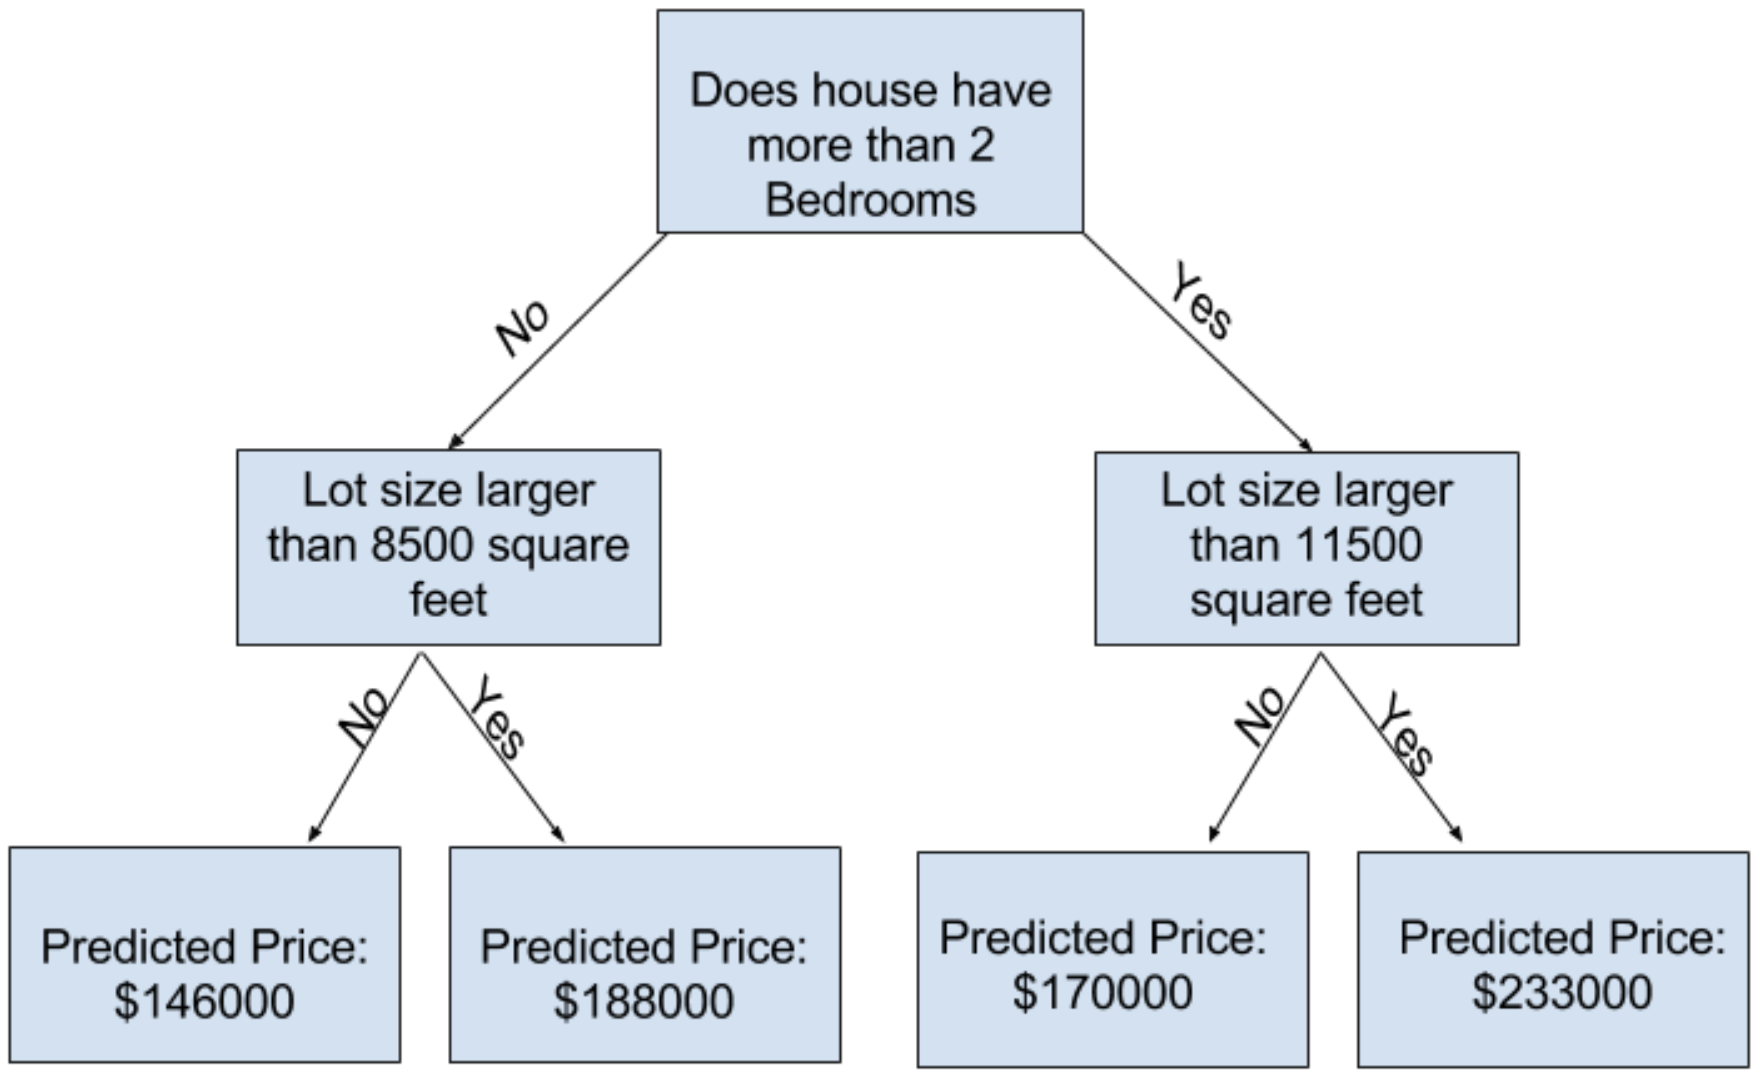
\includegraphics[scale=0.5]{image2.png}

        Deeper Trees
    \end{figure}

    \subsection{Model Validation.}\label{subsec:model_validation}
    You'll want to evaluate almost every model you ever build.
    In most (though not all) applications, the relevant measure of model quality is \textbf{predictive accuracy}.
    In other words, will the model's \textit{predictions be close to what actually happens}.

    There are many metrics for summarizing model quality, but we'll start with one called \textbf{Mean Absolute Error} (also called \textbf{MAE}).

    The prediction error for each house is:
    \[error=actual-predicted\]
    So, if a house cost \$150,000 and you predicted it would cost \$100,000 the error is \$50,000.
    With the MAE metric, we take the \textit{absolute value} of each error.
    This converts each error to a positive number.
    We then take the average of those absolute errors.
    This is our measure of model quality.
    In plain English, it can be said as

    On average, our predictions are off by about X.

    To calculate MAE, we first need a model.
    That is built in a hidden cell below, which you can review by clicking the code button.

    \begin{lstlisting}[style=light, language=Python,label={lst:vectorimg},caption=The mean absolute error calculcation]
        from sklearn.metrics import mean_absolute_error

        predicted_home_prices = melbourne_model.predict(X)
        print(mean_absolute_error(y, predicted_home_prices))
        # 434.71594577146544
    \end{lstlisting}

    \subsection{The Problem with "In-Sample" Scores}\label{subsec:in_sample_problem}
    The measure we just computed can be called an "in-sample" score.
    We used a single "sample" of houses for both building the model and evaluating it.

    The model will appear accurate in the training data.
    But if this pattern doesn't hold when the model sees new data, the model would be very inaccurate when used in practice.

    Since models' practical value come from making predictions on new data, we measure performance on data that wasn't used to build the model.
    The most straightforward way to do this is to exclude some data from the model-building process, and then use those to test the model's accuracy on data it hasn't seen before.
    This data is called \textbf{validation data}.

    \begin{lstlisting}[style=light, language=Python,label={lst:vectorimg},caption=The mean absolute error calculcation]
        from sklearn.model_selection import train_test_split

        # split data into training and validation data, for both features and target
        # The split is based on a random number generator. Supplying a numeric value to
        # the random_state argument guarantees we get the same split every time we
        # run this script.
        train_X, val_X, train_y, val_y = train_test_split(X, y, random_state = 0)
        # Define model
        melbourne_model = DecisionTreeRegressor()
        # Fit model
        melbourne_model.fit(train_X, train_y)

        # get predicted prices on validation data
        val_predictions = melbourne_model.predict(val_X)
        print(mean_absolute_error(val_y, val_predictions))
        # 263007.8766946417
    \end{lstlisting}

    \subsection{Underfitting and Overfitting}\label{subsec:underfitting_overfitting}
    In practice, it's not uncommon for a tree to have 10 splits between the top level (all houses) and a leaf.
    As the tree gets deeper, the dataset gets sliced up into leaves with fewer houses.
    If a tree only had 1 split, it divides the data into 2 groups.
    If each group is split again, we would get 4 groups of houses.
    Splitting each of those again would create 8 groups.
    If we keep doubling the number of groups by adding more splits at each level, we'll have \(2^10\) groups of houses by the time we get to the 10th level.
    That's 1024 leaves.

    When we divide the houses amongst many leaves, we also have fewer houses in each leaf.
    Leaves with very few houses will make predictions that are quite close to those homes' actual values, but they may make very unreliable predictions for new data (because each prediction is based on only a few houses).

    This is a phenomenon called \textbf{overfitting}, where a model matches the training data almost perfectly, but does poorly in validation and other new data.
    On the flip side, if we make our tree very shallow, it doesn't divide up the houses into very distinct groups.

    At an extreme, if a tree divides houses into only 2 or 4, each group still has a wide variety of houses.
    Resulting predictions may be far off for most houses, even in the training data (and it will be bad in validation too for the same reason).
    When a model fails to capture important distinctions and patterns in the data, so it performs poorly even in training data, that is called \textbf{underfitting}.

    Since we care about accuracy on new data, which we estimate from our validation data, we want to find the sweet spot between underfitting and overfitting.
    Visually, we want the low point of the (red) validation curve in

    \subsection{Selecting best number of leaf nodes}\label{subsec:selecting_number_of_leafs}
    There are a few alternatives for controlling the tree depth, and many allow for some routes through the tree to have greater depth than other routes. But the max_leaf_nodes argument provides a very sensible way to control overfitting vs underfitting. The more leaves we allow the model to make, the more we move from the underfitting area in the above graph to the overfitting area.

    We can use a utility function to help compare MAE scores from different values for max\_leaf\_nodes.

    Of the options listed, 500 is the optimal number of leaves.

    \begin{lstlisting}[style=light, language=Python,label={lst:vectorimg},caption=Computing MAE for different value of leaf nodes]
        from sklearn.metrics import mean_absolute_error
        from sklearn.tree import DecisionTreeRegressor

        def get_mae(max_leaf_nodes, train_X, val_X, train_y, val_y):
            model = DecisionTreeRegressor(max_leaf_nodes=max_leaf_nodes, random_state=0)
            model.fit(train_X, train_y)
            preds_val = model.predict(val_X)
            mae = mean_absolute_error(val_y, preds_val)
            return(mae)

        # compare MAE with differing values of max_leaf_nodes
        for max_leaf_nodes in [5, 50, 500, 5000]:
            my_mae = get_mae(max_leaf_nodes, train_X, val_X, train_y, val_y)
            print("Max leaf nodes: %d  \t\t Mean Absolute Error:  %d" %(max_leaf_nodes, my_mae))

        # Max leaf nodes: 5  		 Mean Absolute Error:  347380
        # Max leaf nodes: 50  		 Mean Absolute Error:  258171
        # Max leaf nodes: 500  		 Mean Absolute Error:  243495
        # Max leaf nodes: 5000       Mean Absolute Error:  254983
    \end{lstlisting}


    Models can suffer from either:
    \begin{itemize}
        \item \textbf{Overfitting}: capturing spurious patterns that won't recur in the future, leading to less accurate predictions, or
        \item \textbf{Underfitting}: failing to capture relevant patterns, again leading to less accurate predictions.
    \end{itemize}
    We use validation data, which isn't used in model training, to measure a candidate model's accuracy.
    This lets us try many candidate models and keep the best one.


    \section{Random Forest Tree}\label{sec:random_forest_tree}
    Decision trees leave you with a difficult decision.
    A deep tree with lots of leaves will overfit because each prediction is coming from historical data from only the few houses at its leaf.
    But a shallow tree with few leaves will perform poorly because it fails to capture as many distinctions in the raw data.

    Even today's most sophisticated modeling techniques face this tension between underfitting and overfitting.
    But, many models have clever ideas that can lead to better performance.
    We'll look at the \textbf{random forest} as an example.

    The random forest uses many trees, and it makes a prediction by averaging the predictions of each component tree.
    It generally has much better predictive accuracy than a single decision tree and it works well with default parameters.
    If you keep modeling, you can learn more models with even better performance, but many of those are sensitive to getting the right parameters.

    There is likely room for further improvement, but this is a big improvement over the best decision tree error of 250,000.
    There are parameters which allow you to change the performance of the Random Forest much as we changed the maximum depth of the single decision tree.
    But one of the best features of Random Forest models is that they generally work reasonably even without this tuning.

    \begin{lstlisting}[style=light, language=Python,label={lst:vectorimg},caption=Random Forest Tree]
        from sklearn.ensemble import RandomForestRegressor
        from sklearn.metrics import mean_absolute_error

        forest_model = RandomForestRegressor(random_state=1)
        forest_model.fit(train_X, train_y)
        melb_preds = forest_model.predict(val_X)
        print(mean_absolute_error(val_y, melb_preds))
        # 191669.7536453626
    \end{lstlisting}


\end{document}
